\documentclass{article}
\usepackage[english]{babel}
\usepackage[utf8]{inputenc}
\usepackage{interval}
\usepackage{array}
\usepackage[table]{xcolor}
\usepackage{graphicx}
\usepackage{listings}
\usepackage{hyperref}
\usepackage{amssymb}
\usepackage{multicol}
\usepackage{amsmath, amsthm, amssymb, calrsfs, wasysym, verbatim, bbm, color, graphics, geometry}
\usepackage{graphicx}
\usepackage{float}
\usepackage{rotating}
\usepackage{adjustbox}
\usepackage{booktabs}
\usepackage{caption}
\usepackage{multicol}
\usepackage{amsmath}
\usepackage{minted}


\DeclareMathOperator*{\argmax}{arg\,max}
\DeclareMathOperator{\EX}{\mathbb{E}}% expected value

\hypersetup{
	colorlinks,
	citecolor=black,
	filecolor=black,
	linkcolor=black,
	urlcolor=black
}
\DeclareUnicodeCharacter{2212}{-}
\begin{document}


\begin{titlepage}
      \centering
      \begin{figure}
            \begin{center}
                  
\includegraphics[width=0.6\textwidth]{img/logo_polimi.png}
            \end{center}
      \end{figure}
      \vfill
      {\scshape\LARGE Online Learning Application\\Academic Year 2021 - 2022 \par}
      
      
      \vfill
      \newcommand{\HRule}{\rule{\linewidth}{0.3mm}}
      \centering
      \HRule \\[0.4cm]
      \huge  Pricing \& Social Influence\\% Title of your document
      \HRule \\
      \vspace{1cm}
      {\Large Sofia \textsc{Martellozzo} \quad  Vlad Marian \textsc{Cimpeanu}  \quad  Lorenzo \textsc{Rossi}\par}
      {\Large(10623060) \quad (cod persona) \quad (10698834) \par}
      \vfill
      {\large Professor\par
          Nicola \textsc{Gatti}}
\end{titlepage}


\newpage
\renewcommand\contentsname{Contents}
\tableofcontents

\newpage

%------------------------------------------%
\section*{Introduction}
%where we describe the problem we have to face
Nowadays one big problem of e-commerces is to allocate the best price to its products so that,
the seller can maximize its revenue.\\
The main issue is that increasing the price of a product leads to less people interested in that product, thus
increasing the price is not necessarily beneficial to the seller. In contrast decreasing the price will increase the number
of people interested in the product, but the revenue will be of course sub-optimal.\\
In order to maximize the revenue we can analyze the demand curve of a given product, which is
a graphical representation of the relationship between the price $p_i$ of a good or service $i$ and the quantity demanded $q_i(p_i)$
for a given period of time, and find the price $\hat{p}$ such that:
\begin{align*}
    \hat{p} = \argmax_p(pq(p))
\end{align*}
Unfortunately, in real world problems, the demand curve is not available, furthermore, we need to estimate this curve by interacting with the environment. One main problem of interacting with an unknown environment is that exploration costs a lot of money, so we want to find the best prices in the shortest amount of time to decrease the regret. \\
In order to do so, we can use reinforcement learning techniques such as Multi Armed Bandit (MAB) algorithms.
\subsection*{Practical example}
In this project we want to study the case of a new e-commerce entering the market called ANS$^2$ that sells skateboarding clothes. More precisely, it is going to sell unisex t-shirts, hoodies, t-shirts, shoes and shirts.\\ For simplicity sake we can assume the website can sell an unlimited number of units without any storage cost whose goal is to minimize the cumulative regret while learning.\\
The web site of the vendor is structured as follows: in every webpage, a single product, called primary, is displayed together with its price. The user can add a number of units of this product to the cart. After the product has been added to the cart, two products, called secondary, are recommended. When displaying the secondary products, the price is hidden. Furthermore, the products are recommended in two slots, one above the other, thus providing more importance to the product displayed in the slot above. The website will propose only products that the customer has never seen before.
If the user clicks on a secondary product, a new tab on the browser is opened and, in the loaded webpage, the clicked product is displayed as primary together with its price.\\
The choice of the products that must be recommended to the user are already fixed by the business unit as presented in Figure~\ref{fig:business_graph}.\\\\
\begin{figure}
    \centering
    \includegraphics[scale=0.4]{img/products/business_graph.png}
    \caption{Recommendation graph set by the business unit.}
    \label{fig:business_graph}
\end{figure}
One main consideration we want to make is that the customer may buy different products during a visit, thus the price for a specific product may influence the total income generated by the customer.\\ For instance, let us assume that a customer lands on the webpage displaying a t-shirt: if the price is too high, the probability to buy that product is lower, but not only, also the probability to see the secondary products is lower, so it will decrease the probability that a customer visits and buys new products. In conclusion, when we choose the price for a specific product we have also to consider the indirect reward it will generate.


\newpage
%------------------------------------------%
\section{Step : Environment}
The main aim of the environment is to simulate a real-world scenario. To simulate all the components we divide the model into various classes.
\begin{itemize}
    \item Environment class: It is the wrapper that manages the environment and all its functions. There are two specializations of this class created for some specific use cases (which are EnvironmentContextual and EnvironmentNonStationary).
    \item Simulator class: It manages the simulation of the customers' interactions.
    \item Customer class: It contains all the information that defines a type of customer.
\end{itemize}

\subsection{Parameters}
The environment has a lot of parameters and each of them has a direct and significant impact on the behavior of the model.
Some of the parameters are specifics of the environment:
\begin{itemize}
  \item \verb|customers_distribution| is a list of 4 floating values, that sum to 1. It indicates the probability of each type of customer appearing.
  \item \verb|customer_per_day| is the average number of customers in a day.
  \item \verb|variance_customers| is the standard deviation of the number of customers in a day.
  \item \verb|products_graph| is the graph that indicates which is the primary and secondary product.
  \item \verb|p_lambda| is the probability of observing each slot. The first value is 1, while the second is a number smaller than 1.
  \item \verb|prices| indicates the reward for each product and each price level. Therefore, it is a 4 x 5 matrix.
\end{itemize}
Additionally, some parameters are specifics of the customer:
\begin{itemize}
    \item \verb|features| is the pair of binary features. In our case, the first feature is associated with gender whereas the second one with the age (for simplicity young/old).
    \item \verb|alpha| is a vector that contains the probability distribution of starting from each product.
    \item \verb|buy_distribution| is a matrix containing for each pair (product, price) that defines the probability of buying products.
    \item \verb|num_prods_distribution| is a matrix containing for each pair (product, price), and it controls the number of units the customer is likely to buy for that specific product. In this case, we have decided to model the customer's behavior with a geometric distribution. Thus, they are the \(p\) parameters of the geometric distributions, which is the inverse of the means.
    The main idea behind the geometric distribution is that is a discrete distribution and is monotonically decreasing: the higher the number of products bought, the lower will be the probability to buy that amount of units.
    \item \verb|click_graph| is the probability of clicking the product given a selected price and type of product.
\end{itemize}

\subsection{Learner interaction}
The main aim of the learner is to minimize the cumulative regret by selecting the best price levels.
Therefore, at the beginning of each day, the learner selects the price levels (which is the super arm), and then at the end of the day, it will obtain a report containing all the information about the customer activities, i.e. number of times bought, number of products seen, number of customers.


\subsection{Customer interaction}
The customer interaction works in the following manner:
\begin{enumerate}
    \item Depending on the \verb|alpha| distribution a starting point is randomly chosen.
    \item The customer opens the page and she will buy one or more products with a probability depending on \verb|buy_distribution|. If she does not buy the simulation stops, otherwise the number of items bought is sampled from a geometrical distribution.
    \item Then, with a probability that depends on \(\lambda\) and the \verb|click_graph|, she explores a different product. However, if she has already seen this product, she will not open that page.
\end{enumerate}

From step 3 to step 6 the main assumption is that we have different classes of customers interacting with the website, and each of them has a different behavior. For each step, we know the distribution of the customers and some characteristics of them (for instance the mean of the number of items a customer buys for a specific product), but the website is not able to identify the customer is interacting with it, thus we are not able to estimate the unknown parameters for each customer but only an aggregated estimate.

\subsection{Selection of the super arm}
Since we have to take into consideration also the indirect income generated by other products that are bought after buying the first product, we have to find the combination of prices such that it maximizes the overall income considering the indirect margins, thus we have to solve a combinatorial problem to select the best super arm to play.\\
In order to do so, we have to compute the believed expected reward $\EX\left[ r_a\right]$ for each superarm $a$ and choose the arm with the highest expected reward. We compute the expected reward as follows:
\begin{align*}
    \EX\left[ r_a\right] = \sum_{i \in \mathcal{C}} r_{a,i} w_i
\end{align*}
where $\mathcal{C}$ is the set of indexes of customers, $r_{a,i}$ is the expected reward given the super arm $a$ for customer $i$ and $w_i$ is the probability to see customer $i$.\\
\subsubsection{Monte Carlo methods}
A way to compute the expected reward for a given customer $i$ is to use a Monte Carlo simulation.\\ Monte Carlo methods, or Monte Carlo experiments, are a broad class of computational algorithms that rely on repeated random sampling to obtain numerical results. The underlying concept is to use randomness to solve problems that might be deterministic in principle.\\ Basically, we have 5 seeds (the products) and we run $N$ simulations starting from each seed.
A seed is a starting node in a graph, whose edges $e_{i, j}$ represent the probability of clicking product $j$ given that product $i$ has been bought, whereas each node has an activation threshold that coincides with the probability of buying that product.\\
The simulation works as follows:
\begin{enumerate}
    \item Explore the simulation graph in a depth first search tree fashion. If a node has been already visited, it can not be reached anymore.
    \item When selecting a node $j$, draw a sample $x$ from a Bernoulli distribution  $\mathcal{B}e(t_{i, p, j})$ where $t_{i, p, j}$ is the probability that customer $i$ buys product $j$ at price $p$. If $x < t_{i, p, j}$, activate node $j$, otherwise stop the branch.\\ We can keep track of the number of times a node $j$ has been activated with the variable $\Lambda_j$.
    \item When expanding an active node $i$ towards node $j$, draw a sample $x$ from a Bernoulli distribution $\mathcal{B}e(e_{i, j})$. If $x < e_{i, j}$ move towards node $j$, otherwise stop the branch.
\end{enumerate}
Once a node is activated we draw a sample $n$ from the distribution of the number of items bought for that node (product). Every time a product is bought, we update the number of times that product has been bought:
\begin{align*}
    n_{a, p} = n_{a, p} + n
\end{align*}
where $n_{a, p}$ is the current number of units bought for product $p$ given the super arm $a$.\\
Here, the code for a single simulation:\\
\begin{minted}[breaklines]{python}
def shopping_dfs(self, primary, displayed_primary, report, super_arm, c):
  displayed_primary[primary] = True
  report.seen(primary)
  if np.random.random() < c.get_probability_buy(primary, super_arm[primary]):
    amount = c.get_num_prods(primary, super_arm[primary]) #1
    report.bought(primary, amount)
    click_prob = [c.get_probability_click(primary, secondary) for secondary in self.products_graph[primary]]
    for secondary, edge_prob, lamb in zip(self.products_graph[primary], click_prob, lamb_SLOTS):
      if not displayed_primary[secondary] and np.random.random() < lamb * edge_prob:
        report.move(primary, secondary)
        self.shopping_dfs(secondary, displayed_primary, report, super_arm, c)
\end{minted}
Finally, we compute the expected reward as:
\begin{align*}
    r_{a, i} = \frac{1}{N}\sum_{p \in \mathcal{P}}\alpha_{i, p} a_{p} n_{a, p}
\end{align*}
where $\mathcal{P}$ is the set of indexes of the products, $\alpha_{i, p}$ is the probability for customer $i$ to start from the seed $p$ and $a_{p}$ is the price selected for the product $p$. We can also compute the activation probability (probability that a specific item is bought) of each product as:
\begin{align*}
    \pi_{p, i} = \frac{1}{N}\sum_{p \in \mathcal{P}}\alpha_{i, p} \Lambda_p
\end{align*}
Thanks to the following theorem we have some theoretical guarantees on the accuracy of this method.
\paragraph{Theorem}
With a probability of at least $1 - \delta$, the estimated activation probability of every node is subject to an additive error of $\pm \epsilon n$ when the number of repetitions is:
\begin{align*}
    R = O(\frac{1}{\epsilon^2}log(\mid S \mid)log(\frac{1}{\delta}))
\end{align*}
where $S$ is the number of seeds (5) and $n$ is the number of nodes in the graph (still 5).\\

In our case, if we want to have an additive error of $\epsilon n = 0.1$ ($\epsilon = 0.02$) with a probability of 90 \% ($\delta=0.1$), we need to run $R=1748$, thus the number of simulations for each product for each customer is $N=350$.
In conclusion, this method is stochastic and very noisy, and to obtain a decent estimate we need to run a massive number of simulations which makes the simulation process astonishingly slow.\\
Given the size of the parameters for this problem, we can afford to compute the exact value for the expected value for a given arm in a reasonable time with a different approach.

\subsubsection{Dynamic programming approach}
To overcome the limitation of the Monte Carlo simulation we develop a dynamic programming solution that returns the expected number of items bought. This method has a time complexity of \(\Theta(2^{N}NM)\), where \(N\) is the number of items and \(M\) is the number of types of customers, therefore, this solution is only feasible because the number of items is quite small.
\begin{minted}[breaklines]{python}
def run_dp(self, super_arm):
  ans = 0
  for c, p in zip(self.customers, self.customers_distribution):
    @lru_cache(maxsize=None)
    def dp(primary, mask):
      mask |= 1 << primary
      ans = np.zeros(5)
      ans[primary] = 1 / c.num_prods_distributions[primary][super_arm[primary]]
      click_prob = [c.get_probability_click(primary, secondary) for secondary in self.products_graph[primary]]
      for secondary, edge_prob, lamb in zip(self.products_graph[primary], click_prob, lamb_SLOTS):
        if (mask & (1 << secondary)) == 0:
          ans += lamb * edge_prob * dp(secondary, mask)
      ans *= c.get_probability_buy(primary, super_arm[primary])
      return ans
    for primary, alpha in enumerate(c.get_distribution_alpha()):
      ans += p * alpha * dp(primary, 0)
  return ans
\end{minted}
\subsection{Assumptions}
In this section we list the main assumptions we undertook to face this problem:
\begin{itemize}
    \item for simplicity we assume that the value $\lambda$ for the second displayed product is equal to 1 without loss of generality.
    \item The probability $\alpha_0$ which is the probability to land on another website is omitted, since it does not add any additional feature to the problem.
    \item Customers, accordingly to their behaviour can be grouped into three classes:
    \begin{enumerate}
        \item Boys
        \item Girls
        \item Adults
    \end{enumerate}
    Note: this is just an assumption used to model the customer of the environment, the learner is not acknowledged about this assumption.
\end{itemize}



\newpage
%------------------------------------------%
\section{Step : Optimization algorithm}
Here we consider the case in wich all the parameters are known and the goal is to maximize the cumulative expected reward, following a greedy approach.\\
The algorithm works as follow:
\begin{enumerate}
    \item set the prices of all the pruducts with the lowest one
    \item collect the reward obtained by increasing, each time, the price of just one product of the original super arm
    \item compare the five different configuration obtained with the first one. There could be two case\begin{enumerate}
        \item there is an increase of the reward, so select the one that gave the maximum reward (the highest increase) as the best one and repeat the algorithm from point 2
        \item there is no increse (all the new configuration is worst than the previous one) and stop the algoritm 
    \end{enumerate}
    \item Return the actual best configuration.
\end{enumerate}
For example:\\
The algorithm starts with the super arm with all the lowest prices for all the products : $[0 0 0 0 0]$\\
Then explore by pulling the five combination of super arm, found by increasing of just one one product at time: \\
$[0 0 {\bf1} 0 0]$\\
$[0 0 0 0 {\bf1}]$\\
$[0 0 0 {\bf1} 0]$\\
$[{\bf1} 0 0 0 0]$\\
$[0 {\bf1} 0 0 0]$\\
Now select the one with the highest reward, compare also with the originel best one. In our case it was: $[0 0 0 0 1]$\\ Update the new super arm as the best one and start again, looking at the new five configuration available:\\
$[0 0 0 0 {\bf2}]$\\
$[0 0 {\bf1} 0 {\bf1}]$\\
$[0 {\bf1} 0 0 {\bf1}]$\\
$[{\bf1} 0 0 0 {\bf1}]$\\
$[0 0 0 {\bf1} {\bf1}]$\\
And so on, until no improvement is found.
\subsection{Limitations}
This type of learner do not directly consider the parameters of a Customer, it just interacts with the environment by selecting the arm to pull at each round and observing the reward gibven by the environment.\\
Is guaranteed that the algorithm would not cycle, because it monotonically increases the prices (as well as the cumulative expected margin). On the other hand there is not guarantee that the algorithm will return the optimal price configuration.








\subsection{Results}
\begin{multicols}{2}
    \begin{figure}[H]
        \begin{center}
        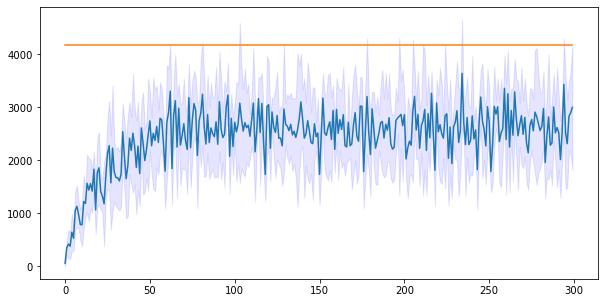
\includegraphics[width=0.5\textwidth]{img/reward2.png}
        \caption{Reward}
        \label{fig:reward2}
        \end{center}
    \end{figure}
    \columnbreak
As said before here we can see\\ that the algorithm converge to a solution\\ that is not optimal,\\ so return a reward that is lower \\than the best possible one (clairvoyant)
\end{multicols}

\begin{multicols}{2}
    \begin{figure}[H]
        \begin{center}
        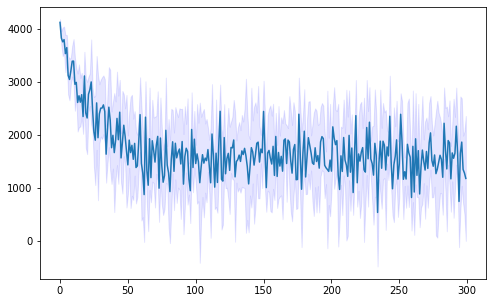
\includegraphics[width=0.5\textwidth]{img/regret2.png}
        \caption{Regret}
        \label{fig:regret2}
        \end{center}
    \end{figure}
    \columnbreak
    \begin{figure}[H]
        \begin{center}
        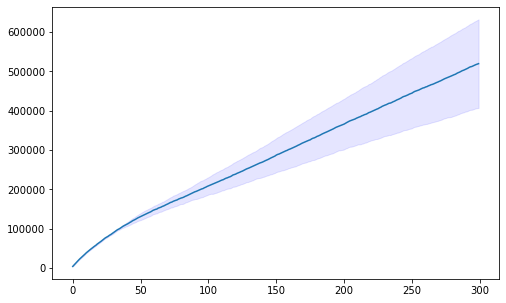
\includegraphics[width=0.5\textwidth]{img/cum_regret2.png}
        \caption{Cumulative regret}
        \label{fig:cum_reg2}
        \end{center}
    \end{figure}
\end{multicols}
As expected the cumulative reward is linear (Figure 3)



\newpage
%------------------------------------------%
\section{Step : Optimization with uncertain conversion rates}
\subsection{Results}
\begin{figure}[ht]
    \begin{center}
    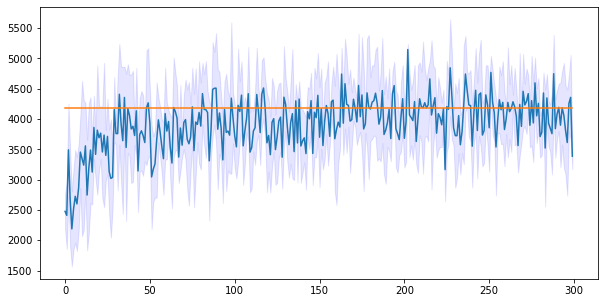
\includegraphics[width=0.6\textwidth]{img/ucb3.png}
    \caption{UCB Reward}
    \label{fig:reward31}
    \end{center}
\end{figure}
\begin{multicols}{2}
    \begin{figure}[H]
        \begin{center}
        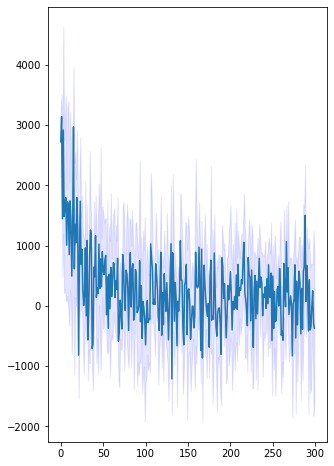
\includegraphics[width=0.5\textwidth]{img/ucb3_regret.png}
        \caption{UCB Regret}
        \label{fig:regret31}
        \end{center}
    \end{figure}
    \columnbreak
    \begin{figure}[H]
        \begin{center}
        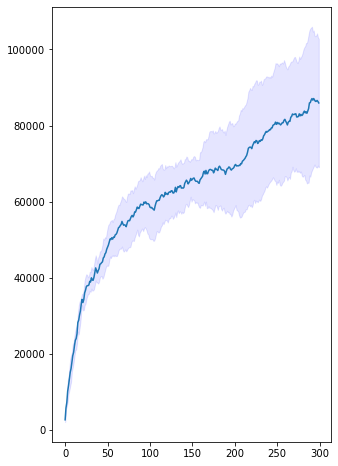
\includegraphics[width=0.5\textwidth]{img/ucb3_cum_reg.png}
        \caption{UCB Cumulative regret}
        \label{fig:cum_reg31}
        \end{center}
    \end{figure}
\end{multicols}
\begin{figure}[ht]
    \begin{center}
    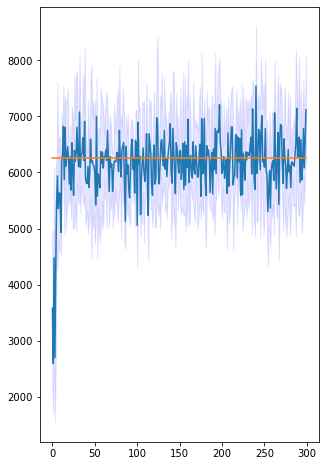
\includegraphics[width=0.6\textwidth]{img/TS3.png}
    \caption{TS Reward}
    \label{fig:reward32}
    \end{center}
\end{figure}
\begin{multicols}{2}
    \begin{figure}[H]
        \begin{center}
        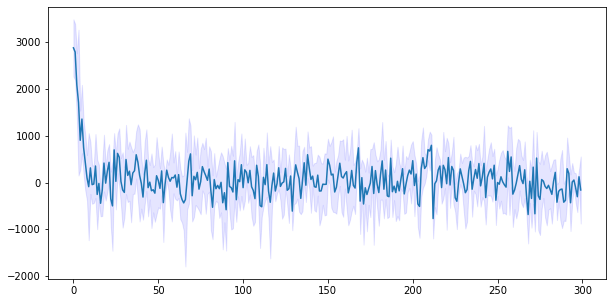
\includegraphics[width=0.5\textwidth]{img/TS3_regret.png}
        \caption{TS Regret}
        \label{fig:regret32}
        \end{center}
    \end{figure}
    \columnbreak
    \begin{figure}[H]
        \begin{center}
        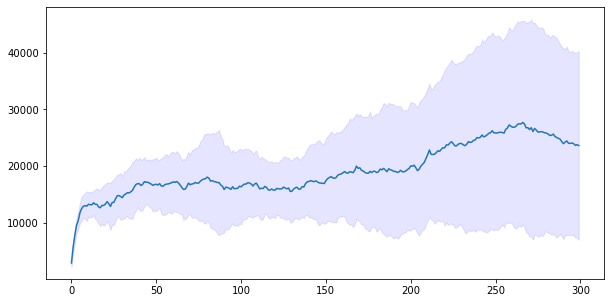
\includegraphics[width=0.5\textwidth]{img/TS3_cum_reg.png}
        \caption{TS Cumulative regret}
        \label{fig:cum_reg32}
        \end{center}
    \end{figure}
\end{multicols}


\newpage
%------------------------------------------%
\section{Step : Optimization with uncertain conversion rates, $\alpha$ ratios, and number of items sold per product}
Here the problem is the same as in the previous step, with the only difference being that also the alpha ratios and the number of products sold for each price are unknown.
Since the learners are not able to distinguish the different types of customers, initially the alphas values (probability to start the interaction from a specific product) are uniformly distributed ($[0.2, 0.2, 0.2, 0.2, 0.2]$) and the number of products bought for each price is set all to 1.\\
The same algorithms as before have been developed, with the additional calculus to estimate the two parameters, now uncertain.

\subsection{UCB-1}
The algorithm repeats the same operations as in the previous chapter from step 1 to step 5. Then, it estimates the two parameters:

\begin{itemize}
    \item estimate alpha ratios $\alpha_{i, t}$:
    \begin{align}
        \sigma_{i, t} = \sigma_{i, t - 1} + starts_{i, t}, \forall i \in \mathcal{P}\\
        \alpha_{i, t} = \frac{\sigma_{i, t}}{\sum_{j \in \mathcal{P}}\sigma_{j, t}},  \forall i \in \mathcal{P}
        \label{eqn:alpha}
    \end{align}Where:\begin{itemize}
        \item $\sigma_{i, t}$ is the number of starts from product $i$ has been observed until time $t$
        \item $starts_{i, t}$ is the number of starting times observed at time $t$ for product $i$
        \item $\mathcal{P}$ is the set of indexes for the products
        \end{itemize}
    \item estimate number of products sold (version 1):\\
    with this first approach, we evaluate these parameters with the empirical mean as can be seen in Equation ~\ref{eqn:num_prod} \begin{equation}
        \label{eqn:mean_items}
        mean\_items[p,a] = \frac{mean\_items[p,a] * seen[p,a] + bought[p]}{estimated\_items[p,a]}
    \end{equation}\begin{equation}
        \label{eqn:num_prod}
        num\_products[p,a] = \frac{1}{mean\_items[p,a]}
    \end{equation}where\begin{itemize}
        \item mean\_items[p,a] is the mean of the number of products {\bf p} with price {\bf a} bought until now
        \item seen[p,a] is the number of times product {\bf p} with price {\bf a} has been bought until the day before
        \item bought[p] is the total amount of products {\bf p} bought on the current day
        \item estimated\_items[p,a] is the number of times products {\bf p} with price {\bf a} have been bought until now (so it is seen[p,a] plus the number of times product p has been bought the current day)
        \item num\_products[p,a] is the inverse of the value computed before because represents the parameter of the Geometric distribution, which we have used to estimate the number of items bought by the customers, once they have decided to buy that product visualized with that price.
    \end{itemize}
    \item estimate number of products sold (version 2):\\
    Since the number of units bought by a customer depends on the price (so, by the chosen arm), we try to use a UCB-1 algorithm to estimate also this parameter. UCB-1 relies on the assumption that the variable we want to estimate has support in $\left[0, 1 \right]$, but the number of units bought belongs to $\left[0, +\infty \right)$, thus we can not directly estimate the number of units with this algorithm.\\
    One possibility is to directly evaluate the parameter of the Geometric distribution (the inverse of the mean). Normally, UCB-1 uses the upper bound to give an optimistic estimate of the parameters in order to induce the exploration of new arms. However, since increasing the parameter of the Geometric distribution will lead to a decrement in the believed estimation of the number of units bought, we will get a pessimistic estimate. To overcome this issue, we subtract the upper bound from the mean, instead of adding.\\
 The results of this version are significantly worse and are not shown below.
\end{itemize}
\subsubsection{Results}
As expected, having less knowledge leads to a solution a little bit worse than the previous step. In other words, the UCB Learner needs more days to converge to the optimal solution. As said before, someday it will change the super arm to pull, in order to explore more.
\begin{figure}[ht]
    \begin{center}
    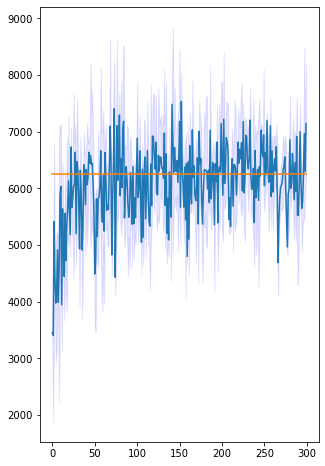
\includegraphics[width=0.6\textwidth]{img/UCB4.png}
    \caption{UCB Reward}
    \label{fig:reward41}
    \end{center}
\end{figure}
\begin{multicols}{2}
    \begin{figure}[H]
        \begin{center}
        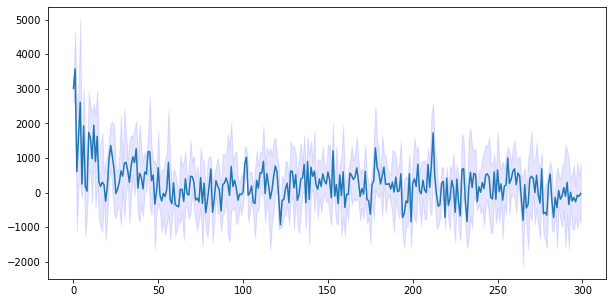
\includegraphics[width=0.5\textwidth]{img/UCB4_regret.png}
        \caption{UCB Regret}
        \label{fig:regret41}
        \end{center}
    \end{figure}
    \columnbreak
    \begin{figure}[H]
        \begin{center}
        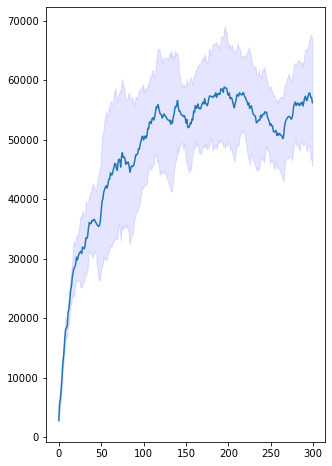
\includegraphics[width=0.5\textwidth]{img/UCB4_cum_reg.png}
        \caption{UCB Cumulative regret}
        \label{fig:cum_reg41}
        \end{center}
    \end{figure}
\end{multicols}

\subsection{TS}
Thomson Sampling estimates the alpha ratios exactly as the UCB with the Equation ~\ref{eqn:alpha}.\\About the estimation of the number of products sold, the method adopted is the same as the second version for the UCB-1. For obvious reasons, the additional parameters are the $\alpha$ and $\beta$ parameters of the Beta distribution used for the additional MAB. The update of $\alpha$ is done as follows:
\begin{align*}
    \alpha[p, a] = \alpha[p, a] + tot\_bought[p]
\end{align*}
where tot\_bought [p] is the total amount of products {\bf p} bought from the first day until now, whereas the update of the $\beta$ parameters is:
\begin{align*}
    \beta[p, a] = \beta [p, a] + seen[p]
\end{align*}
where seen [p] is the number of times the product {\bf p} has been bought until now.\\\\
The two parameters calculated above are updated in the customer's attributes when the learner has to select which super arm to pull.\\

\subsubsection{Results}
The same results as UCB can be observed here, more uncertainty leads to more time to converge. Also this time the results highlight the fact that TS performs better than UCB because it takes less time to converge, generating less cumulative regret.\\ Furthermore, the reason why using the Thompson Sampling algorithm to estimate both the conversion rate and the number of units sold is more effective than UCB-1 might be because it is less explorative. Having two UCB-1 algorithms may lead to too much exploration and less exploitation.
\begin{figure}[ht]
    \begin{center}
    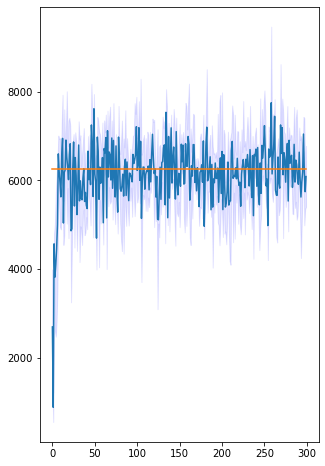
\includegraphics[width=0.6\textwidth]{img/TS4.png}
    \caption{TS Reward}
    \label{fig:reward42}
    \end{center}
\end{figure}
\begin{multicols}{2}
    \begin{figure}[H]
        \begin{center}
        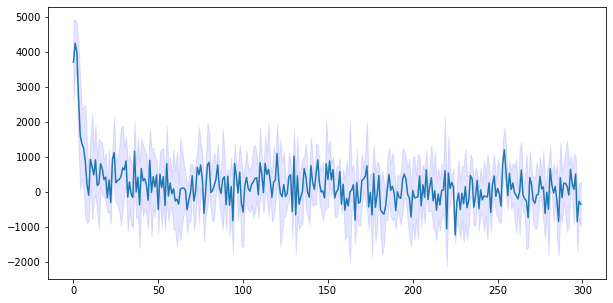
\includegraphics[width=0.5\textwidth]{img/TS4_regret.png}
        \caption{TS Regret}
        \label{fig:regret42}
        \end{center}
    \end{figure}
    \columnbreak
    \begin{figure}[H]
        \begin{center}
        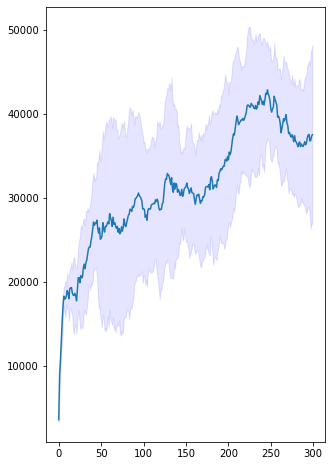
\includegraphics[width=0.5\textwidth]{img/TS4_cum_reg.png}
        \caption{TS Cumulative regret}
        \label{fig:cum_reg42}
        \end{center}
    \end{figure}
\end{multicols}


\newpage
%------------------------------------------%
\section{Step : Optimization with uncertain graph weights}
Consider now the case in which, as in step 3, the conversion rates are unknown but also the values of the graph weights.\\ These parameters gave us the probability that a customer clicks on the secondary product having a given product as primary.\\ Therefore, we initialize both learners (UCB-1 and TS) with the graph weights all set to 1.\\ 
In the same way as the previous step, below are reported only the addictional calculus to estimate the new unknown parameters.

\subsection{UCB-1}
As said before the first five step are the same, so here is reported how the graph weights are estimated:
\begin{equation}
    estimated\_graph[p,:] = \frac{estimated\_graph[p,:] * bought[p] + clicks[p,:]}{tot\_bought[p]}
\end{equation}Where: \begin{itemize}
    \item estimated\_graph[p,:] is the vector of all the weights of the graph that starts from the node with the product {\bf p}
    \item bought[p] is the number of times the product {\bf p} has been bought until the day before
    \item clicks[p,:] is the row of the matrix that reports the number of times an edge of the graph has been activated, that means that a click on the secondary product (columns) has been recorded given a primary product (row). So here we look at all the edge that has been activated starting by the primary profuct {\bf p}
    \item tot\_bought[p] is the number of times the product {\bf p} has been bought until today (so it is bought[p] plus the number of times product p has been bought today)
\end{itemize}
\subsection{TS}
In this case the Thomson Sampling does exactly the same as the UCB-1 to estimate the graph weights.
\subsection{Results}
Also in this case the results are very similar to the previous step: both algorithms perform a little bit worse than the case in which only one parameter was uncertain (conversion rates).\\ Another thing that remains unchanged is that TS performed better than UCB-1 by reaching the optimal super arm faster.
\begin{figure}[ht]
    \begin{center}
    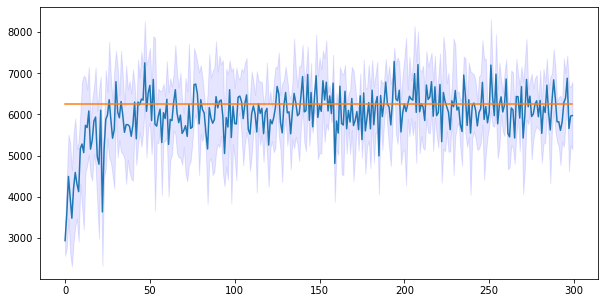
\includegraphics[width=0.6\textwidth]{img/ucb_reward5.png}
    \caption{UCB Reward}
    \label{fig:reward51}
    \end{center}
\end{figure}
\begin{multicols}{2}
    \begin{figure}[H]
        \begin{center}
        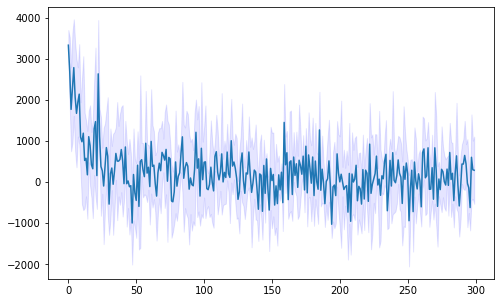
\includegraphics[width=0.5\textwidth]{img/ucb_regret5.png}
        \caption{UCB Regret}
        \label{fig:regret51}
        \end{center}
    \end{figure}
    \columnbreak
    \begin{figure}[H]
        \begin{center}
        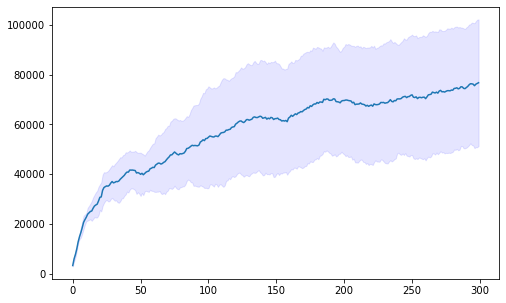
\includegraphics[width=0.5\textwidth]{img/ucb_cum_regret5.png}
        \caption{UCB Cumulative regret}
        \label{fig:cum_reg51}
        \end{center}
    \end{figure}
\end{multicols}
\begin{figure}[ht]
    \begin{center}
    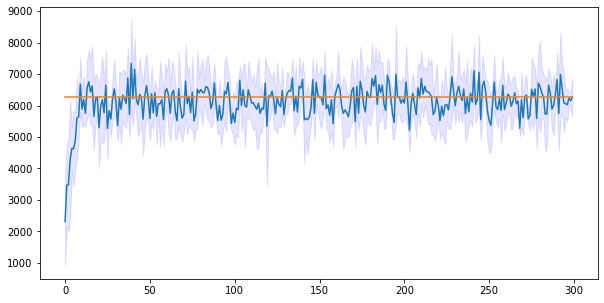
\includegraphics[width=0.6\textwidth]{img/ts_reward5.png}
    \caption{TS Reward}
    \label{fig:reward52}
    \end{center}
\end{figure}
\begin{multicols}{2}
    \begin{figure}[H]
        \begin{center}
        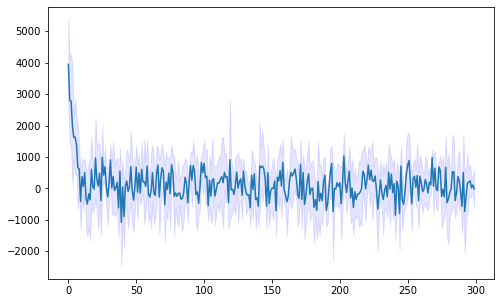
\includegraphics[width=0.5\textwidth]{img/ts_regret5.png}
        \caption{TS Regret}
        \label{fig:regret52}
        \end{center}
    \end{figure}
    \columnbreak
    \begin{figure}[H]
        \begin{center}
        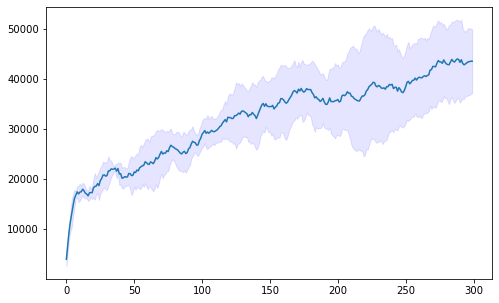
\includegraphics[width=0.5\textwidth]{img/ts_cum_regret5.png}
        \caption{TS Cumulative regret}
        \label{fig:cum_reg52}
        \end{center}
    \end{figure}
\end{multicols}

\newpage
%------------------------------------------%
\section{Step : Non-stationary demand curve}
In this section we face the case in which the demand curves are unknown and can be subject to abrupt changes. More precisely, our proposed simulator present an abrupt change every 100 days involving the demand curves for each product for each customer.
We use different approaches to face the same problem:
\begin{itemize}
    \item UCB-1 algorithm with abrupt change detection.
    \item UCB-1 algorithm with sliding window.
\end{itemize}
\subsection{Abrupt change detection}
\label{learner2}
In this case, at the end of each day, the learner, before updating its arms, checks either the conversion rate has changed or not for each product for each price. The naivest way is to compute the conversion rate of the current day $\alpha_t(p, a)$ for product $p$ given price $a$ and compare it with the average of the conversion rates of the last days $\hat{\alpha}_{t-1}(p, a)$.\\ We set a threshold $\delta$ such that if :
\begin{align*}
        \alpha_t(p, a) \not\in \left[ \hat{\alpha}_{t-1}(p, a) - \delta, \hat{\alpha}_{t-1}(p, a) + \delta \right]
\end{align*}
then that specific conversion rate has just changed. Due to the high noise that characterizes the realizations of the environment it is incredibly hard to understand why a realization might be out of the range.
\\In order to overcome this issue we propose a slightly advanced approach: instead of comparing the last conversion rate with the average of the last conversion rates, we say that the conversion rate for a specific product for a given price has changed if:
\begin{align*}
    \hat{\alpha}_{t, t -\lambda}(p, a) \not\in \left[ \hat{\alpha}_{t-\lambda, 1}(p, a) - \delta, \hat{\alpha}_{t-\lambda, 1}(p, a) + \delta \right]
\end{align*}
where $\hat{\alpha}_{t, t -\lambda}(p, a)$ is the average of the last $\lambda$ conversion rates, whereas $ \hat{\alpha}_{t-\lambda, 1}(p, a)$ is the average of the first $t - \lambda$ conversion rates for that product $p$ at price $a$. This method reveals to be more robust to the noise of the environment, but requires more days to detect an anomaly, nevertheless, we can achieve great results setting $\lambda$ to 5 as we can see from Figures~\ref{fig:reward61}, \ref{fig:regret61}, \ref{fig:cum_reg61}.\\
Once a conversion rate has been spotted as changing, all the data related to that specific pair (price, arm) are dropped, since those data are no more relevant.\\
Here the code for the detection algorithm:
\begin{minted}[breaklines]{python}
    def change_detection_test(self, pulled_arm, report):
        conv_rate = report.get_conversion_rate()
        for product, arm in enumerate(pulled_arm):
            delta = 0.3
            mean1, mean2 = 0, 0

            if len(self.conv_rate_history[product][arm]) > 10:
                last_conv_rates = self.conv_rate_history[product][arm][-self.splitter:]
                last_conv_rates.append(conv_rate[product])

                mean1 = np.mean(self.conv_rate_history[product][arm][:-self.splitter])

                mean2 = np.mean(last_conv_rates)

            if self.t_arms[product, arm] > 11 and (mean1 < mean2 - delta or mean1 > mean2 + delta) and not np.isinf(
                    self.upper_bounds[product, arm]):
                # detected an abrupt change
                self.t_arms[product, arm] = 0
                self.means[product, arm] = 0
                self.upper_bounds[product, arm] = np.inf
                self.seen[product, arm] = 0
                self.conv_rate_history[product][arm] = [conv_rate[product]]
\end{minted}
\subsection{Insights on abrupt change detection algorithm}
\label{learner1}
Now we want to investigate and understand if under the assumption to already know all the conversion rates will change, we can improve the performance of the learner: when a change for a single pair (price, product) is detected, all the conversion rates are dropped. From Figures~\ref{fig:reward62}, \ref{fig:regret62}, \ref{fig:cum_reg62} we notice the two algorithms have comparable performances, thus, there is no reason to use a more specific algorithm as the one just introduced.

\subsection{Sliding window}
Finally we change the UCB-1 algorithm implementing the sliding window to keep track of the most relevant samples.
The main idea behind this algorithm is the demand curves are currently smoothly changing, thus samples loose importance with the time.\\
In order to avoid old samples to affect the learner's performance, we use a sliding window of size $\sigma$: in other words we compute the estimated conversion rates and their upper bounds using only the last $\sigma$ samples.\\
The drawback of sliding window is the learner has a short memory about the past, thus, if it is used on a stationary environment, it it will be outperformed by a stationary UCB-1 algorithm, since it will behave in a more exploratory way.
Using a sliding window of size 50, we can see from Figures~\ref{fig:reward63}, \ref{fig:regret63}, \ref{fig:cum_reg63}, the learner with the change detection algorithm outperforms
the one using the sliding window. This should not surprise us for the following reasons:
\begin{itemize}
    \item Our environment is characterized by three stationary phases. When a change occurs, it is abrupt instead of being smooth: sliding window has been thought to face the second scenario, thus it will be slower to converge.
    \item For the first 100 days, the environment is stationary, thus the sliding window struggle to converge since it is discarding the oldest samples, despite they are still useful.
\end{itemize}




\subsection{Results}
In this subsection we present the experimental results got interacting with a non stationary environment for 300 days and the number of daily customers is drawn every day from a Normal distribution $\mathcal{N}(300, 10)$.
\begin{figure}[ht]
    \begin{center}
    \includegraphics[width=0.6\textwidth]{img/rewards_active2.png}
    \caption{Change detection UCB Reward}
    \label{fig:reward61}
    \end{center}
\end{figure}
\begin{multicols}{2}
    \begin{figure}[H]
        \begin{center}
        \includegraphics[width=0.5\textwidth]{img/regret_active2.png}
        \caption{Change detection UCB Regret}
        \label{fig:regret61}
        \end{center}
    \end{figure}
    \columnbreak
    \begin{figure}[H]
        \begin{center}
        \includegraphics[width=0.5\textwidth]{img/cumulative_regret_active2.png}
        \caption{Change detection UCB Cumulative regret}
        \label{fig:cum_reg61}
        \end{center}
    \end{figure}
\end{multicols}

\begin{figure}[ht]
    \begin{center}
    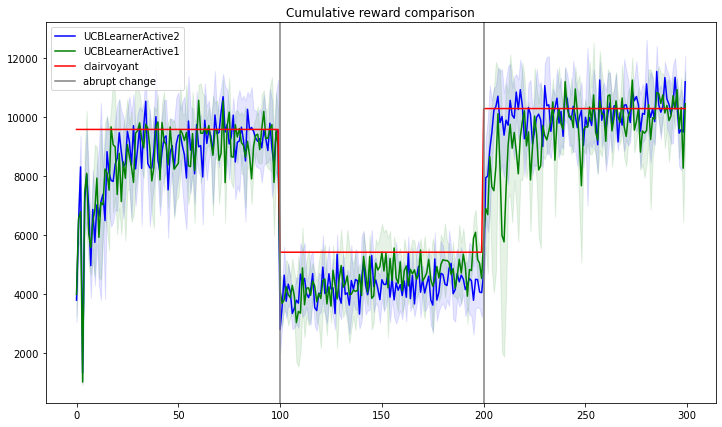
\includegraphics[width=0.6\textwidth]{img/reward_LA1vsLA2.png}
    \caption{Reward comparison between Learner 1 (algorithm in Subsection~\ref{learner1}) and Learner 2 (algorithm in Subsection~\ref{learner2})}
    \label{fig:reward62}
    \end{center}
\end{figure}
\begin{multicols}{2}
    \begin{figure}[H]
        \begin{center}
        \includegraphics[width=0.5\textwidth]{img/regret_LA1vsLA2.png}
        \caption{Regret comparison between Learner 1 (algorithm in Subsection~\ref{learner1}) and Learner 2 (algorithm in Subsection~\ref{learner2})}
        \label{fig:regret62}
        \end{center}
    \end{figure}
    \columnbreak
    \begin{figure}[H]
        \begin{center}
        \includegraphics[width=0.5\textwidth]{img/cumulative_regret_LA1vsLA2.png}
        \caption{Cumulative regret comparison between Learner 1 (algorithm in Subsection~\ref{learner1}) and Learner 2 (algorithm in Subsection~\ref{learner2})}
        \label{fig:cum_reg62}
        \end{center}
    \end{figure}
\end{multicols}


\begin{figure}[ht]
    \begin{center}
    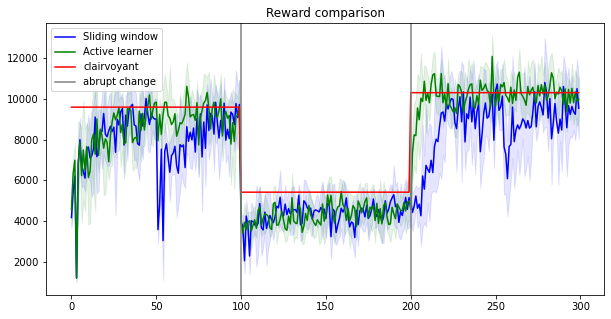
\includegraphics[width=0.6\textwidth]{img/sw_vs_active_reward.png}
    \caption{TODO: CAMBIARE IMMAGINI Reward comparison between Learner with change detection algorithm and Learner with sliding window}
    \label{fig:reward63}
    \end{center}
\end{figure}
\begin{multicols}{2}
    \begin{figure}[H]
        \begin{center}
        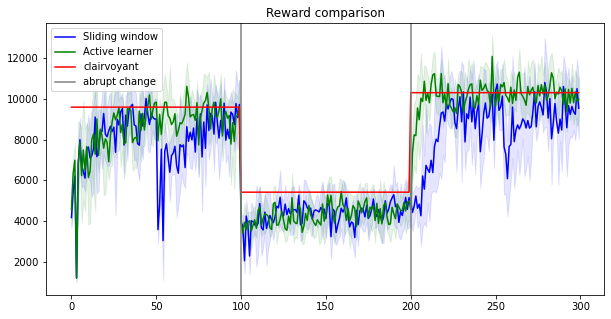
\includegraphics[width=0.5\textwidth]{img/sw_vs_active_reward.png}
        \caption{Regret comparison between Learner with change detection algorithm and Learner with sliding window}
        \label{fig:regret63}
        \end{center}
    \end{figure}
    \columnbreak
    \begin{figure}[H]
        \begin{center}
        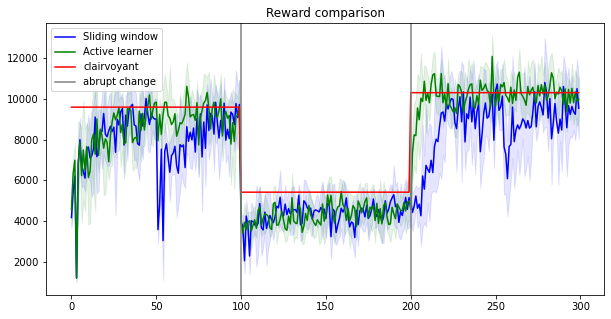
\includegraphics[width=0.5\textwidth]{img/sw_vs_active_reward.png}
        \caption{Cumulative regret comparison between Learner with change detection algorithm and Learner with sliding window}
        \label{fig:cum_reg63}
        \end{center}
    \end{figure}
\end{multicols}



\newpage
%------------------------------------------%
\section{Step : Context generation}
This step is very similar to step 4, however, we can observe the customer features.
Therefore, we can set different price levels for every type of customer.
To leverage this information, every two weeks a context context-generation algorithm is executed.
The algorithm uses a feature tree to select the learner, and it is built using a greedy splitting technique.

\subsection{How to build the feature tree}
Starting from the root node, for each feature the algorithm computes the expected reward without splitting, so by training only a single learner and with splitting on the features, therefore, by training two learners on two partitions of the data.
If the expected reward is larger in the latter case, the node is split in the two cases and the process continues recursively on every new node.

\subsection{Results}
\subsubsection{UCB}
\begin{figure}[ht]
    \begin{center}
    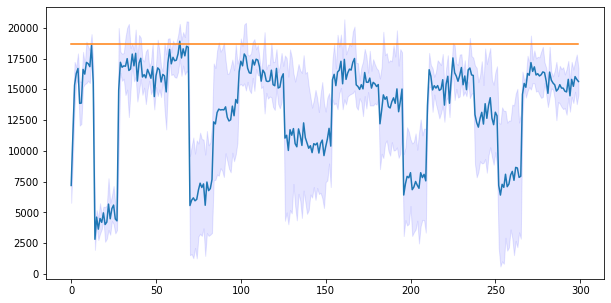
\includegraphics[width=0.6\textwidth]{img/ucb7.png}
    \caption{UCB Reward}
    \label{fig:reward7}
    \end{center}
\end{figure}
\begin{multicols}{2}
    \begin{figure}[H]
        \begin{center}
        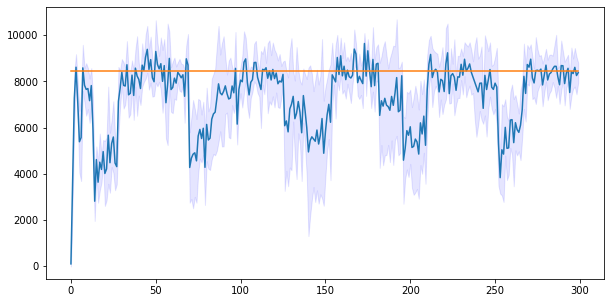
\includegraphics[width=0.5\textwidth]{img/ucb7_1.png}
        \caption{UCB Reward customer 1}
        \label{fig:reward71}
        \end{center}
    \end{figure}
    \columnbreak
    \begin{figure}[H]
        \begin{center}
        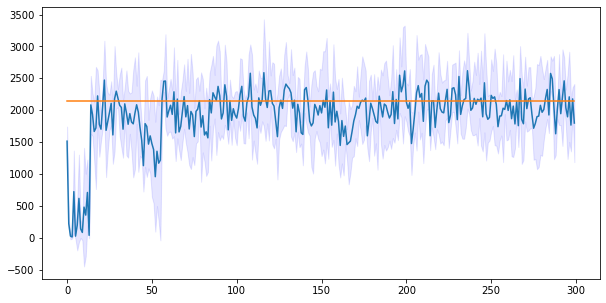
\includegraphics[width=0.5\textwidth]{img/ucb7_2.png}
        \caption{UCB Reward customer 2}
        \label{fig:reward72}
        \end{center}
    \end{figure}
\end{multicols}
\begin{multicols}{2}
    \begin{figure}[H]
        \begin{center}
        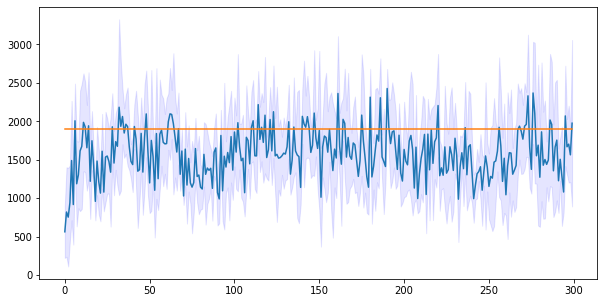
\includegraphics[width=0.5\textwidth]{img/ucb7_3.png}
        \caption{UCB Reward customer 3}
        \label{fig:reward73}
        \end{center}
    \end{figure}
    \columnbreak
    \begin{figure}[H]
        \begin{center}
        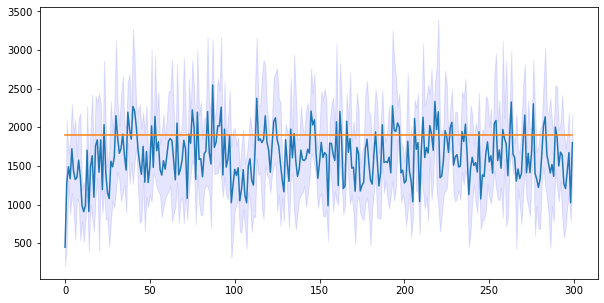
\includegraphics[width=0.5\textwidth]{img/ucb7_4.png}
        \caption{UCB Reward customer 4}
        \label{fig:reward74}
        \end{center}
    \end{figure}
\end{multicols}

\begin{multicols}{2}
    \begin{figure}[H]
        \begin{center}
        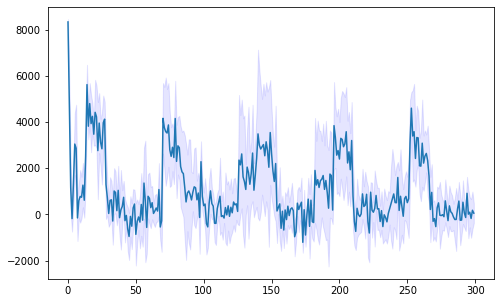
\includegraphics[width=0.5\textwidth]{img/ucb7_1regret.png}
        \caption{UCB Regret customer 1}
        \label{fig:regret71}
        \end{center}
    \end{figure}
    \columnbreak
    \begin{figure}[H]
        \begin{center}
        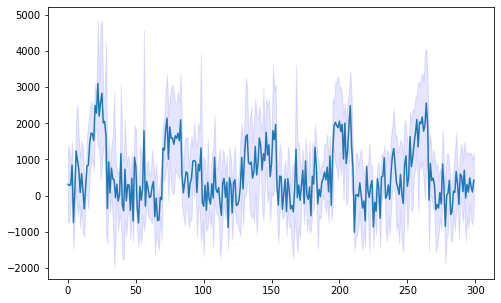
\includegraphics[width=0.5\textwidth]{img/ucb7_2regret.png}
        \caption{UCB Regret customer 2}
        \label{fig:regret72}
        \end{center}
    \end{figure}
\end{multicols}
\begin{multicols}{2}
    \begin{figure}[H]
        \begin{center}
        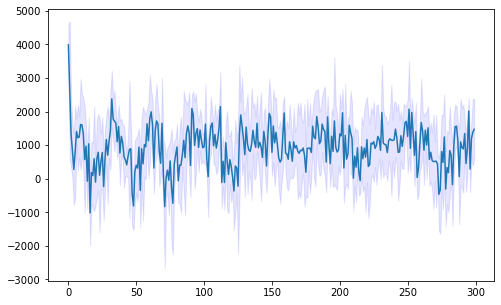
\includegraphics[width=0.5\textwidth]{img/ucb7_3regret.png}
        \caption{UCB Regret customer 3}
        \label{fig:regret73}
        \end{center}
    \end{figure}
    \columnbreak
    \begin{figure}[H]
        \begin{center}
        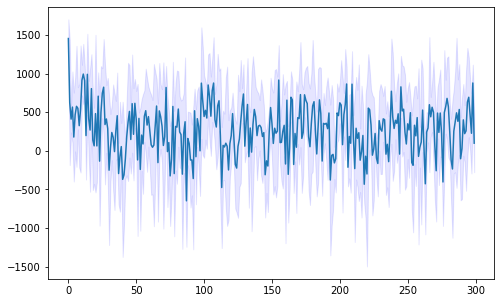
\includegraphics[width=0.5\textwidth]{img/ucb7_4regret.png}
        \caption{UCB Regret customer 4}
        \label{fig:regret74}
        \end{center}
    \end{figure}
\end{multicols}

\begin{multicols}{2}
    \begin{figure}[H]
        \begin{center}
        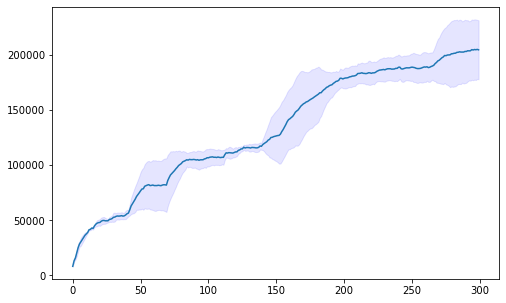
\includegraphics[width=0.5\textwidth]{img/ucb7_1cum_reg.png}
        \caption{UCB Cumulative regret customer 1}
        \label{fig:cum_reg71}
        \end{center}
    \end{figure}
    \columnbreak
    \begin{figure}[H]
        \begin{center}
        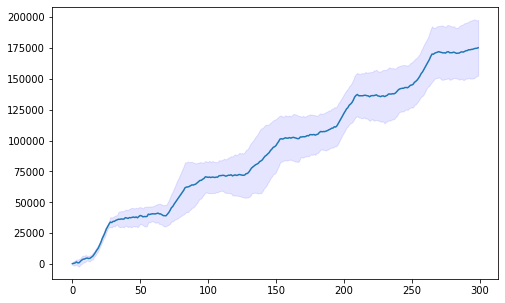
\includegraphics[width=0.5\textwidth]{img/ucb7_2cum_reg.png}
        \caption{UCB Cumulative regret customer 2}
        \label{fig:cum_reg72}
        \end{center}
    \end{figure}
\end{multicols}
\begin{multicols}{2}
    \begin{figure}[H]
        \begin{center}
        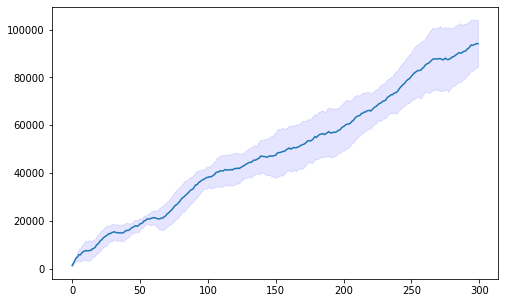
\includegraphics[width=0.5\textwidth]{img/ucb7_3cum_reg.png}
        \caption{UCB Cumulative regret customer 3}
        \label{fig:cum_reg73}
        \end{center}
    \end{figure}
    \columnbreak
    \begin{figure}[H]
        \begin{center}
        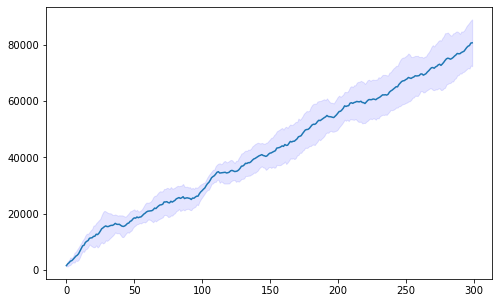
\includegraphics[width=0.5\textwidth]{img/ucb7_4cum_reg.png}
        \caption{UCB Cumulative regret customer 4}
        \label{fig:cum_reg74}
        \end{center}
    \end{figure}
\end{multicols}

\subsubsection{TS}


\end{document}